\documentclass[12pt,a4paper]{article}
\usepackage[top=3cm, includefoot] {geometry} 
\usepackage[utf8]{inputenc}
\usepackage[T1]{fontenc}
\usepackage{lmodern}
\usepackage{amsmath}
\usepackage{amsfonts}
\usepackage{amssymb}
\usepackage[czech]{babel}
\usepackage{graphicx}
\usepackage{epstopdf}
\usepackage{url}
\usepackage{float}
\usepackage{listings}
\usepackage{subfigure}
\usepackage{titling,lipsum}
\usepackage{indentfirst}
\usepackage{hhline}
\usepackage{enumerate}
\usepackage{caption}
\usepackage{pdfpages}
\author{Ondřej Vaníček \and Václav Helma}
\title{Automatické řízení\\Semestrální práce}

\begin{document}
	\pagenumbering{gobble}% Remove page numbers (and reset to 1)
	\clearpage
	\thispagestyle{empty}
	\maketitle
	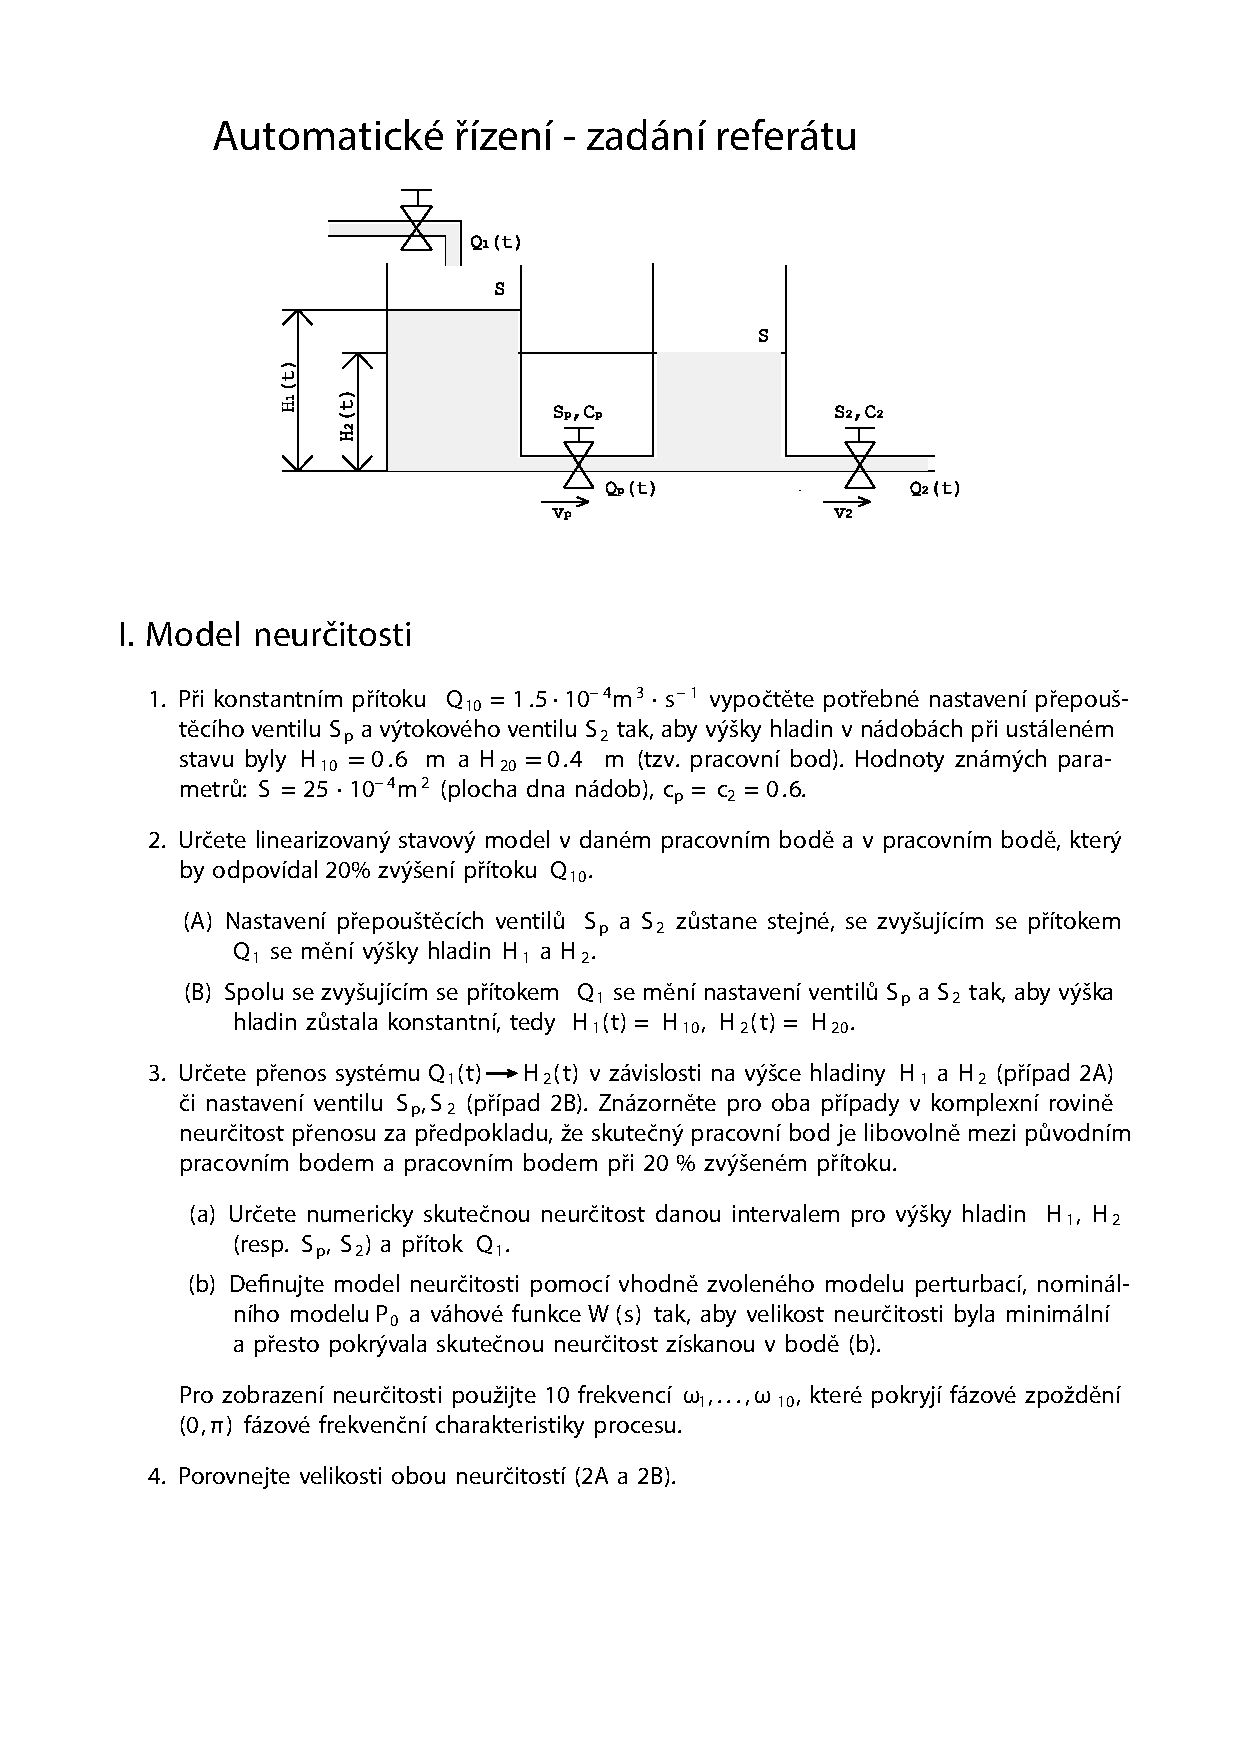
\includepdf[pages={1,2}]{ar1.pdf}
	\newpage
	\pagestyle{plain}
	\pagenumbering{arabic}
	\setcounter{page}{1}
	\section*{Vypracování}
	\begin{enumerate}[I.]
		\item\textbf{Model neurčitosti}
		\begin{enumerate}[1.]
			\item K výpočtu potřebného nastavení ventilů $ S_p $ a $ S_2 $ je nejprve nutné sestavit matematický model dané soustavy.\\
			Označíme-li $ V_1 $ objem kapaliny v 1. nádobce a $ V_2 $ objem kapaliny v 2. nádobce, $ Q_1 $ přítok do 1. nádobky, $ Q_p $ přítok do 2. nádobky a $ Q_2 $ odtok z 2. nádobky, potom můžeme napsat
			\begin{gather*}
			\frac{dV_1}{dt} = Q_1(t) - Q_p(t) \label{dV1},\\
			\frac{dV_2}{dt} = Q_p(t) - Q_2(t) \label{dV2},
			\end{gather*}
			kde $ V_1 $, resp. $ V_2 $ lze zapsat jako
			\begin{gather*}
			V_1 = s \cdot H_1(t) \label{V1},\\
			V_2 = s \cdot H_2(t) \label{V2}
			\end{gather*}
			a $ Q_p $ resp. $ Q_2 $ jako
			\begin{gather*}
			Q_p = S_p \cdot C_p \cdot v_p(t) \label{Qp},\\
			Q_2 = c_2 \cdot S_2 \cdot v_2(t) \label{Q2}.
			\end{gather*}
			Z Bernouliho rovnice lze určit rychlosti $ v_p $ a $ v_2 $, tedy rychlost přítoku do 2. nádobky a rychlost výtoku z 2. nádobky
			\begin{gather*}
			v_p(t) = \sqrt{2\cdot g\cdot(H_1(t)-H_2(t))} \label{vp},\\
			v_2(t) = \sqrt{2\cdot g\cdot H_2(t)} \label{v2}.
			\end{gather*}
			Z těchto vztahů získáme
			\begin{gather}
			\frac{dH_1(t)}{dt} = \frac{Q_1(t)}{S} - \frac{C_p \cdot S_p}{S} 
			\cdot \sqrt{2g \cdot (H_1(t) - H_2(t)} \label{dH1},\\
			\frac{dH_2(t)}{dt} = \frac{C_p \cdot S_p}{S} \cdot \sqrt{2g \cdot (H_1(t) - H_2(t))} - \frac{C_2 \cdot S_2}{S} \cdot \sqrt{2g\cdot H_2(t)} \label{dH2}.
			\end{gather}
			Z těchto rovnic nyní vypočítáme potřebné nastavení ventilů, aby se soustava dostala do požadovaného ustáleného stavu. Definice ustáleného stavu praví, že ustává veškerý pohyb v dynamice systému (při konstantním vstupu $ Q_{1konst} $), což znamená, že derivace jsou rovny nule. Můžeme tedy počítat
			\begin{gather*}
			0 = \frac{Q_1(t)}{S} - \frac{C_p \cdot S_p}{S} \cdot \sqrt{2g \cdot (H_1(t) - H_2(t)},\\
			0 = \frac{C_p \cdot S_p}{S} \cdot \sqrt{2g \cdot (H_1(t) - H_2(t))} - \frac{C_2 \cdot S_2}{S} \cdot \sqrt{2g\cdot H_2(t)},
			\end{gather*}
			z čehož vyjádříme
			\begin{gather}
			S_p = \frac{Q_{1konst}}{C_p\cdot \sqrt{2g(H_1 - H_2)}} \label{Sp},\\
			S_2 = \frac{ C_p\cdot S_p \sqrt{H_1 - H_2}}{C_2\sqrt{H_2}} \label{S2}
			\end{gather}
			a konečně po dosazení všech hodnot ($Q_{1konst} = 1,5 \cdot 10^{-4}  m^3 \cdot s^{-1}, h_1 = 0,6 m, h_2 = 0,4m, S = 25 \cdot 10^{-4}m^2, C_p=C_2=0,6 $) získáme
			\begin{gather}
			S_p = 1,2620 \cdot 10^{-4} \label{SpF},\\
			S_2 = 8,9240 \cdot 10^{-5} \label{S2F}.
			\end{gather}
			\item Linearizovaný stavový model daného systému určíme pomocí Taylorova polynomu prvního stupně, tudíž matice dynamiky $ A $ a matice řízení $ B $ budou vypadat následovně
			\begin{gather*}
			A = \left[\begin{array}{cc}
				\frac{\partial f_1}{\partial H_1} & \frac{\partial f_1}{\partial H_2} \\
				\frac{\partial f_2}{\partial H_1} & \frac{\partial f_2}{\partial H_2}
			\end{array}\right],
			B = \left[\begin{array}{c}
				\frac{\partial f_1}{\partial Q_1} \\
				\frac{\partial f_2}{\partial Q_1}
			\end{array}\right].
			\end{gather*}
			Po provedení jednotlivých parciálních derivací získáme následující podobu matic A a B
			\begin{gather}
			A = \left[\begin{array}{cc}
			-\frac{C_{p}S_{p}\sqrt{2g}}{2\cdot S \sqrt{(H_1 - H_2)}}
			& \frac{C_{p}S_{p}\sqrt{2g}}{2\cdot S \sqrt{(H_1 - H_2)}} \\
			\frac{C_{p}S_{p}\sqrt{2g}}{2\cdot S \sqrt{(H_1 - H_2)}}
			& -\frac{C_{p}S_{p}\sqrt{2g}}{2\cdot S \sqrt{(H_1 - H_2)}} - \frac{C_2\cdot S_2\cdot g}{S\cdot \sqrt{(2gH_2)}}
			\end{array}\right],
			B = \left[\begin{array}{c}
			\frac{1}{S} \\ 0
			\end{array}\right].\label{statespace}
			\end{gather}
			Matice vyčíslíme
			\begin{gather*}
			A = \left[\begin{array}{cc}
				-0,1498 & 0,1498\\
				0,1498 & -0,2248
			\end{array}\right],
			B = \left[\begin{array}{c}
			400 \\ 0
			\end{array}\right].
			\end{gather*}
			Vzhledem k tomu, že jednotlivé stavy jsou zároveň výstupy a vstup přímo neovlivňuje výstup, platí
			\begin{gather*}
			C = \left[\begin{array}{cc}
				1 & 0\\
				0 & 1
			\end{array}\right],
			D = \left[\begin{array}{c}
				0 \\ 0
			\end{array}\right].
			\end{gather*}
			Konečně stavový popis linearizovaného systému je
			\begin{gather}		
			\left[
			\begin{array}{c c}
			\dot{x}_1(t) \\
			\dot{x}_2(t) 
			\end{array}
			\right]
			= 
			\left[\begin{array}{c c}
			-0,1498 & 0,1498\\
			0,1498 &	-0,2248
			\end{array}\right]
			\cdot \left[\begin{array}{c}
			x_1(t) \\
			x_2(t)
			\end{array}\right]
			+ \left[\begin{array}{c}
			400\\
			0
			\end{array}\right]
			\cdot u(t),\nonumber
			\\
			\left[
			\begin{array}{c c}
			y_1(t) \\
			y_2(t) 
			\end{array}
			\right]
			= 
			\left[\begin{array}{c c}
			1 & 0\\
			0 & 1
			\end{array}\right]
			\cdot \left[\begin{array}{c}
			x_1(t) \\
			x_2(t)
			\end{array}\right]. \label{ss_nom}
			\end{gather}
			Nyní přichází na řadu nový pracovní bod, který je dán navýšením přítoku $ Q_1 $ o 20\%. Zvýšený přítok $ Q = Q_{1konst} \cdot 1,2 $. Z rovnic rovnovážného stavu (\ref{Sp}) a (\ref{S2}) odvodíme následující vztahy
			\begin{gather*}
			H_2 = \frac{Q^2}{2g\cdot S_2^2 \cdot c_2^2} \label{H2},\\
			H_1 = \frac{Q^2}{2g\cdot S_p^2 \cdot c_p^2} + H_2. \label{H1}
			\end{gather*}
			Dosazením přítoku a konstant získáme nový pracovní bod $ \left[0,864; 0,576\right] $. Dosazením pracovního bodu do maticové reprezentace (obdobně jako v předchozím případě) získáme nový stavový model pro zvýšený přítok
			\begin{gather}
			\left[
			\begin{array}{c c}
			\dot{x}_1(t) \\
			\dot{x}_2(t) 
			\end{array}
			\right]
			= 
			\left[\begin{array}{c c}
			-0,1248 & 0,1248\\
			0,1248 &	-0,1873
			\end{array}\right]
			\cdot \left[\begin{array}{c}
			x_1(t) \\
			x_2(t)
			\end{array}\right]
			+ \left[\begin{array}{c}
			400\\
			0
			\end{array}\right]
			\cdot u(t),\nonumber
			\\
			\left[
			\begin{array}{c c}
			y_1(t) \\
			y_2(t) 
			\end{array}
			\right]
			= 
			\left[\begin{array}{c c}
			1 & 0\\
			0 & 1
			\end{array}\right]
			\cdot \left[\begin{array}{c}
			x_1(t) \\
			x_2(t)
			\end{array}\right]. \label{ss_1}
			\end{gather}
			Dále je zapotřebí určit linearizovaný stavový model v případě, že přítok je stejně jako v předchozím případě navýšen o 20\%, avšak hladiny zůstávají stejné a mění se nastavení přepouštěcích ventilů. Dosadíme tedy do rovnic (\ref{Sp}) a (\ref{S2}) a dostaneme
			\begin{gather*}
			S_p = 1{,}5145\cdot 10^{-4},\\
			S_2 = 8{,}924\cdot 10^{-5}.
			\end{gather*}
			Nyní dosadíme všechny známe parametry do (\ref{statespace}) dostaneme linearizovaný model
			\begin{gather}
			\left[
			\begin{array}{c c}
			\dot{x}_1(t) \\
			\dot{x}_2(t) 
			\end{array}
			\right]
			= 
			\left[\begin{array}{c c}
			-0,1800 & 0,1800\\
			0,1800 & -0,2550
			\end{array}\right]
			\cdot \left[\begin{array}{c}
			x_1(t) \\
			x_2(t)
			\end{array}\right]
			+ \left[\begin{array}{c}
			400\\
			0
			\end{array}\right]
			\cdot u(t), \nonumber
			\\
			\left[
			\begin{array}{c c}
			y_1(t) \\
			y_2(t) 
			\end{array}
			\right]
			= 
			\left[\begin{array}{c c}
			1 & 0\\
			0 & 1
			\end{array}\right]
			\cdot \left[\begin{array}{c}
			x_1(t) \\
			x_2(t)
			\end{array}\right]. \label{ss_2}
			\end{gather}
			\item Ze stavového popisu (\ref{ss_nom}) lze určit přenos $Q_1(t) \rightarrow H_2(t)$
			\begin{gather*}
			P(s) = \frac{60}{s^2 + 0{,}375s + 0{,}01125}.
			\end{gather*}
			Dále je nutné určit přenosy $Q_1(t) \rightarrow H_2(t)$ ze stavových popisů (\ref{ss_1}) a (\ref{ss_2})
			\begin{gather*}
			P_H = \frac{50}{s^2 + 0{,}3125s + 0{,}007813},\\
			P_S = \frac{72}{s^2 + 0{,}45s + 0{,}0162}.
			\end{gather*}
			Neurčitost daná intervalem za předpokladu, že skutečný pracovní bod je  libovolně mezi původním pracovním bodem a a pracovním bodem při 20\% zvýšeném přítoku a měnících se výškách hladin $P_1$ byla určena z přenosů $P$ a $P_H$
			\begin{gather*}
			P_1(s) = \frac{<50;60>}{s^2 + <0{,}3125;0{,}375>s + <0{,}007813;0{,}01125>}.
			\end{gather*}
			Nadále jsme se zaměřili na určení modelu neurčitosti, v našem případě konkrétně aditivní neurčitosti, pomocí nominálního modelu a váhové funkce
			\begin{gather*}
			P_a(s) = P_{0a}(s) + W_a(s)\Delta,
			\end{gather*}
			kde $||\Delta||_\infty \leq 1$.\\
			Nominálním modelem $P_{0a}(s)$ systému jsme označili přenos při přítoku navýšeném o 10 \%
			\begin{gather*}
			P_{0a} = \frac{54{,}55}{s^2 + 0{,}3409s + 0{,}009298}.
			\end{gather*}
			Váhovou funkci aditivní neurčitosti jsme posléze určili jako rozdíl $W_a(s) = P(s)-P_{0a}(s)$
			\begin{gather*}
			W_a(s) = \frac{5{,}455s^2 + 3{,}553\cdot 10^{-15}s - 0{,}05579}{s^4 + 0{,}7159s^3 + 0{,}1484s^2 + 0{,}007322s + 0{,}0001046}.
			\end{gather*}
			Velikost této neurčitosti pak je jednoduše $|W_a(s)|$.\\
			Nyní tedy můžeme znázornit neurčitost v komplexní rovině. Na obrázku \ref{fig:neurcitost2A} je vykreslena tato neurčitost pro 10 různých frekvencí.
			\begin{figure}[H]
				\centering
				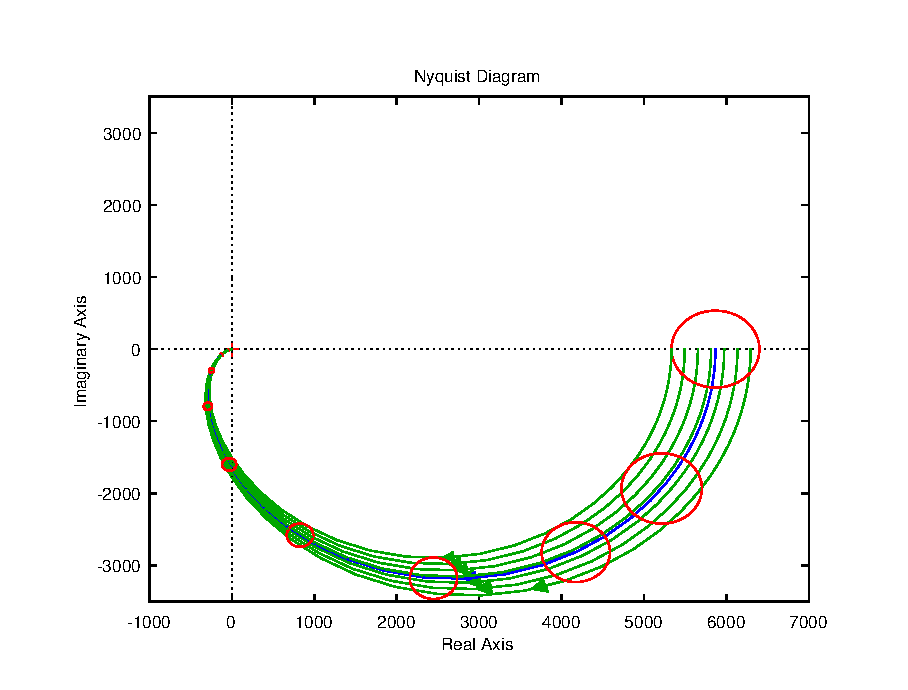
\includegraphics{images/neurcitost1.eps}
				\caption{Neurčitost(bod 2A), modře - nominální přenos, zeleně - perturbované přenosy, červeně - neurčitost}
				\label{fig:neurcitost2A}
			\end{figure}
			Stejný postup lze uplatnit i v dalším případě.
			Neurčitost daná intervalem za předpokladu, že skutečný pracovní bod je libovolně mezi původním pracovním bodem a pracovním bodem při 20\% zvýšeném přítoku a měnícím se nastavením přepouštěcích ventilů $P_2$ byla určena z přenosů $P$ a $P_S$
			\begin{gather*}
			P_2(s) = \frac{<60;72>}{s^2 + <0{,}375;0{,}45>s + <0{,}01125;0{,}0162>}.
			\end{gather*}
			Dále určíme model neurčitosti pomoci nominálního přenosu a váhové funkce
			\begin{gather*}
			P_b(s) = P_{0b}(s) + W_b(s)\Delta.
			\end{gather*}
			Zopakujeme tedy stejný postup jako v předchozím případě a nominálním modelem $P_{0b}(s)$ bude přenos při přítoku navýšeném o 10\%, tentokrát však samozřejmě při měnícím se nastavení přepouštěcích ventilů
			\begin{gather*}
			P_{0b}(s) = \frac{66}{s^2 + 0{,}4125s + 0{,}01361}.
			\end{gather*}
			Aditivní váhovou funkci $W_b(s)$ vypočítáme jako rozdíl $W_b(s) = P(s)-P_{0b}(s)$
			\begin{gather*}
			W_b(s) = \frac{-6s^2 - 3{,}55\cdot 10^{-15}s + 0{,}07425}{s^4 + 0{,}7875s^3 + 0{,}1796s^2 + 0{,}009745s + 0{,}0001531}.
			\end{gather*}
			Na obrázku \ref{fig:neurcitost2B} je tato neurčitost, stejně jako v předchozím případě, znázorněna v komplexní rovině.
			\begin{figure}[H]
				\centering
				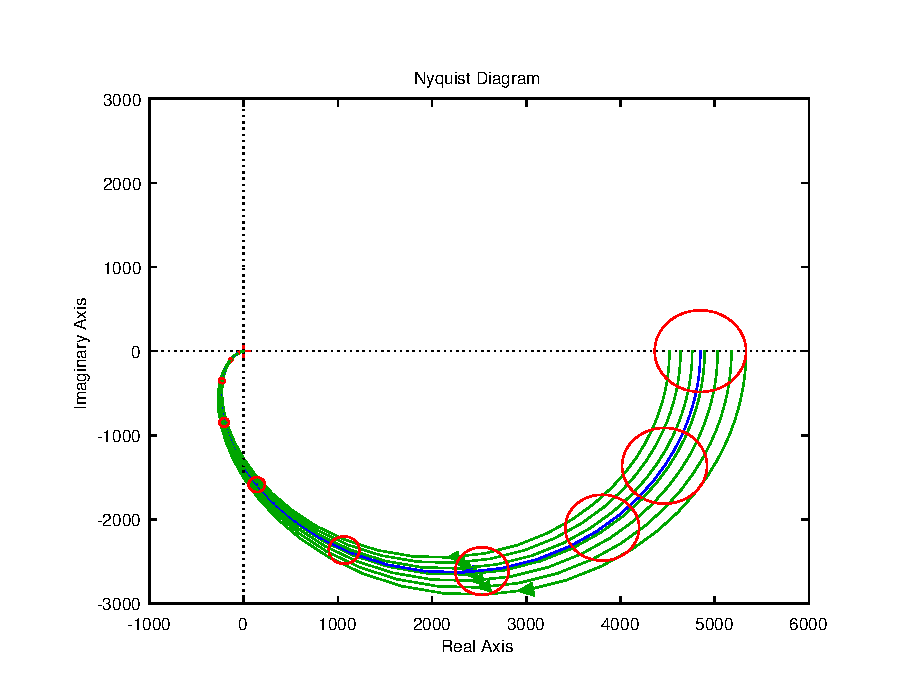
\includegraphics{images/neurcitost2.eps}
				\caption{Neurčitost(bod 2B), modře - nominální přenos, zeleně - perturbované přenosy, červeně - neurčitost}
				\label{fig:neurcitost2B}
			\end{figure}
			\item Na obrázku \ref{fig:velikost_neurcitosti} jsou pomocí Bodeho amplitudové frekvenční charakteristiky porovnány velikosti obou neurčitostí.
			\begin{figure}[H]
				\centering
				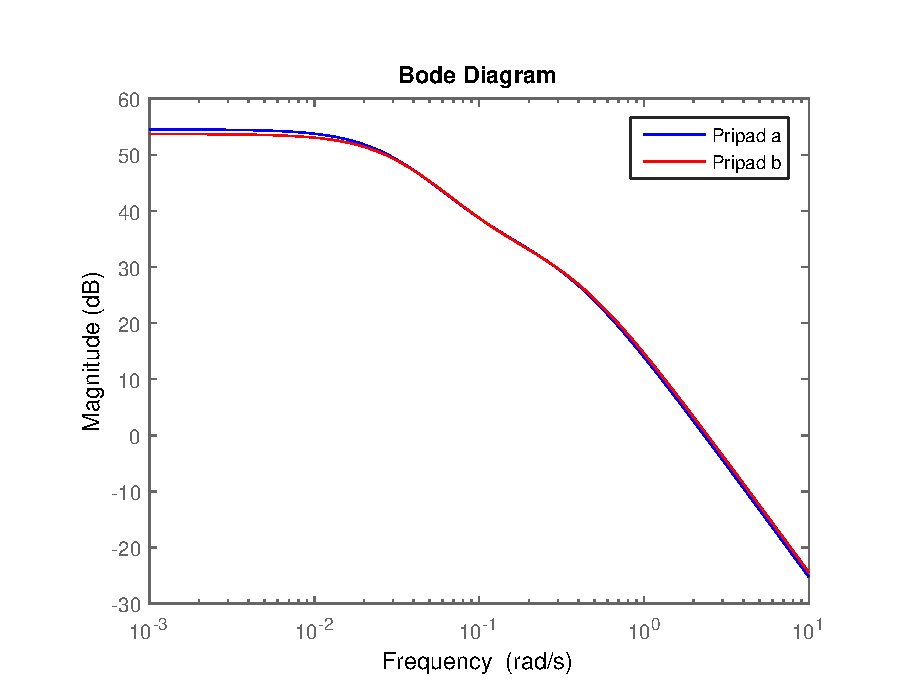
\includegraphics{images/velikost_neurcitosti.eps}
				\caption{Porovnání velikostí obou neurčitostí}
				\label{fig:velikost_neurcitosti}
			\end{figure}
			Z grafu je patrné, že velikosti obou neurčitostí jsou na všech frekvencích velmi podobné.
%			\item V tabulce \ref{tab:neurcitosti} je porovnání velikostí obou neurčitostí.
%			\begin{center}
%				\begin{tabular}{| l || l | l |}
%					\hline
%					 & $|P_1-P_{10}|$ & $|P_2-P_{20}|$\\
%					\hhline{|=|=|=|}
%					$\omega_1$ & $1{,}909.10^{3}$ & $1{,}067.10^{3}$\\
%					\hline
%					$\omega_2$ & $1{,}745.10^{3}$ & $1{,}015.10^{3}$\\
%					\hline
%					$\omega_3$ & $1{,}486.10^{3}$ & $924{,}269$\\
%					\hline
%					$\omega_4$ & $1{,}055.10^{3}$ & $742{,}607$\\
%					\hline
%					$\omega_5$ & $624{,}216$ & $504{,}226$\\
%					\hline
%					$\omega_6$ & $330{,}465$ & $295{,}488$\\
%					\hline
%					$\omega_7$ & $115{,}612$ & $151{,}076$\\
%					\hline
%					$\omega_8$ & $59{,}877$ & $63{,}774$\\
%					\hline
%					$\omega_9$ & $18{,}726$ & $21{,}553$\\
%					\hline
%					$\omega_{10}$ & $5{,}457$ & $6{,}491$\\
%					\hline
%				\end{tabular}
%				\captionof{table}{Porovnání velikostí neurčitostí}
%				\label{tab:neurcitosti}
%			\end{center}
%			Z tabulky je patrné, že první neurčitost je větší než druhá neurčitost na nízkých frekvencích. Naopak na vysokých frekvencích je menší.
		\end{enumerate}
		\item\textbf{Návrh regulátoru}\\
		\begin{enumerate}[1.]
				\item Úkolem druhé části semestrální práce bylo navrhnout parametry PI regulátoru tak, aby byly splněny jisté návrhové požadavky pro všechny systémy z modelu neurčitosti získaného v první části práce, konkrétně se jedná o model, v něž se mění výšky hladin.\\
				Přítok $Q_1(t)$ je realizován vodním čerpadlem. Nejprve je tedy nutné rozšířit přenos systému $P_a(s)$ o aproximovaný model čerpadla $Q_{pump}(s)$, abychom dostali finální model řízené soustavy $P_{cs}$
				{\footnotesize				
				\begin{gather*}
				P_{cs} = Q_{pump}(s)\cdot P_a(s) = \frac{Q_{10}}{0{,}5s + 1}\cdot P_a(s) = \frac{0{,}01636}{s^3 + 2{,}341s^2 + 0{,}6911s + 0{,}0186}.
				\end{gather*}}
				Získali jsme tedy přenos řízeného systému, který je dle zdání třeba řídit PI regulátorem s přenosem
				\begin{gather*}
				C(s) = \frac{Ks + K_i}{s}.
				\end{gather*}
				Po detailnějším prozkoumání problému jsme se rozhodli pro použití konkrétních parametrů $K = 4$ a $K_i = 0{,}3$. Nominální přenos otevřené smyčky, který je potřeba pro další analýzu, má tvar
				\begin{gather*}
				L_0(s) = C(s)\cdot Q_{pump}(s)\cdot P_{0a}(s).
				\end{gather*}
				Uzavřená smyčka pak měla splňovat následující základní požadavky na robustní kvalitu řízení pro všechny systémy z modelu neurčitosti. Systém měl být vnitřně stabilní a amplituda citlivostní funkce nesměla přesáhnout hodnotu $M_s = 2$.\\
				K ověření platnosti těchto předpokladů lze využít vztah pro robustní kvalitu
				\begin{gather*}
				|||W_1(s)S_0(s)| + |W_2(s)T_0(s)|||_\infty < 1,
				\end{gather*}
				kde $S_0(s)$ je nominální citlivostní funkce $S_0(s) = \frac{1}{1 + L_0(s)}$ a $T_0(s)$ je komplementární citlivostní funkce s předpisem $T_0(s) = \frac{L_0(s)}{1+L_0(s)}$.\\
				Funkce $W_2$ je pak určena váhovou funkcí modelu neurčitosti získanou v první části práce $W_2(s) = \frac{W_a(s)}{P_{0a}(s)}$. Funkce $W_1(s)$ je pro náš požadavek na kvalitu řízení jednoduše $W_1(s) = \frac{1}{2}$.\\
				Po výpočtu nekonečno normy jsme obdrželi výsledek
				\begin{gather}
				|||W_1(s)S_0(s)| + |W_2(s)T_0(s)|||_\infty = 0{,}8237. \label{robust_kval}
				\end{gather}
				Vidíme, že uzavřená smyčka splňuje základní požadavky na robustní kvalitu řízení. Tento test (\ref{robust_kval}) lze rovněž ilustrovat graficky pomocí Bodeho amplitudové frekvenční charakteristiky(obrázek \ref{fig:robustni_kvalita}).
				\begin{figure}[H]
					\centering
					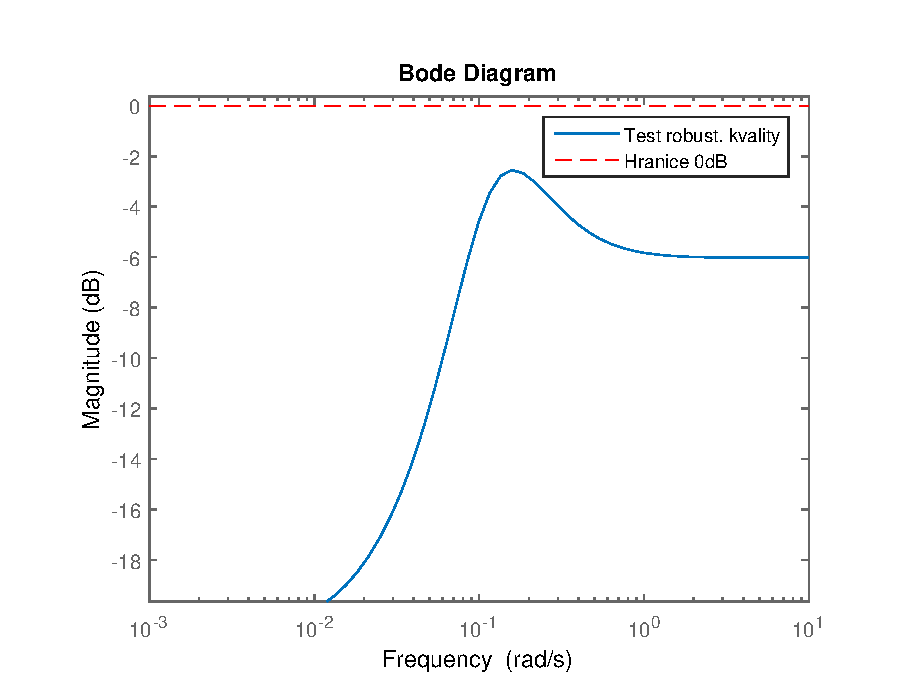
\includegraphics{images/robustni_kvalita.eps}
					\caption{Test robustní kvality}
					\label{fig:robustni_kvalita}
				\end{figure}
				Posléze jsme ještě provedli test stability pomocí Nyquistova kritéria, viz obrázek \ref{fig:nyquist}.
				\begin{figure}[H]
					\centering
					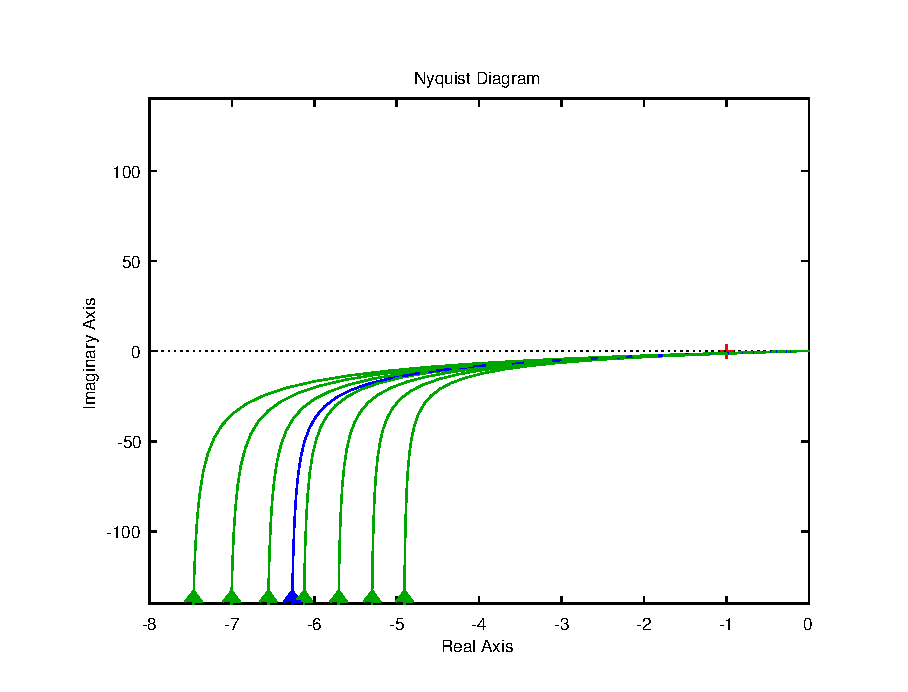
\includegraphics{images/nyquist.eps}
					\caption{Nyquistovo kritérium, modře - nominální přenos, zeleně - perturbované přenosy}
					\label{fig:nyquist}
				\end{figure}
				Vzhledem k následnému testování dalších vlastností uzavřené smyčky, je zde vhodné přiložit Bodeho amplitudové frekvenční charakteristiky nominální citlivostní funkce a komplementární citlivostní funkce(obrázek \ref{fig:citlivostni_funkce}). 
				\begin{figure}[H]
					\centering
					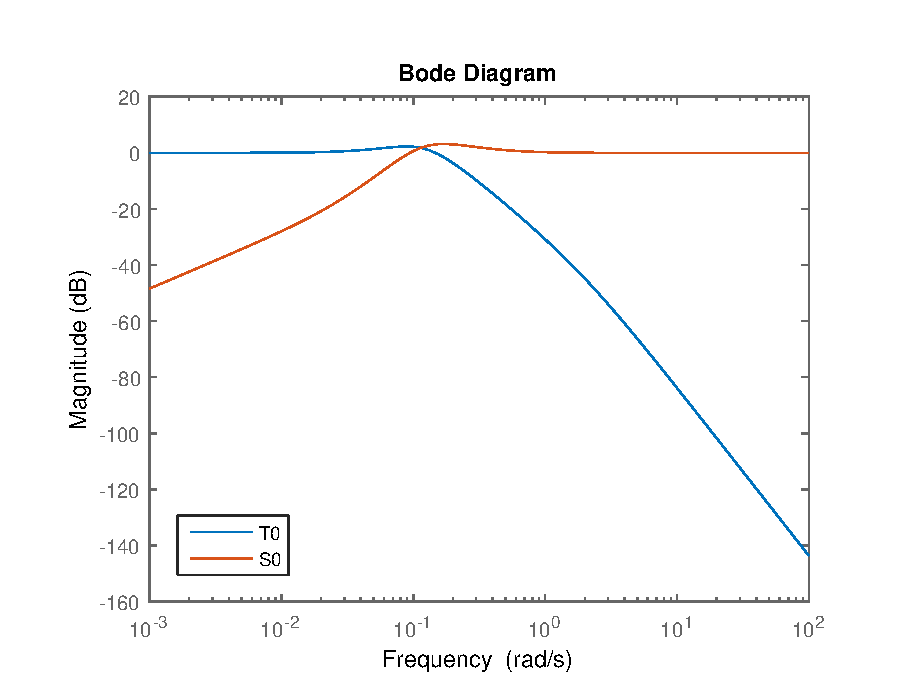
\includegraphics{images/citlivostni_funkce.eps}
					\caption{Nominální citlivostní a komplementární citlivostní funkce}
					\label{fig:citlivostni_funkce}
				\end{figure}
				Kvůli předpokladům ohledně dostupné šířce pásma regulace, bylo dále nutné, aby útlum komplementární citlivostní funkce na frekvenci $\Omega_a = 10 rad/sec$ byl alespoň $-10dB$. Maximální hodnotu amplitudy komplementární citlivostní funkce na dané frekvenci jsme tedy určili takto
				{\footnotesize
				\begin{gather*}
				20\log \left(\left|\frac{C(j10).Q_{pump}(j10).(P_{0a}(j10)+W_a(j10))}{1+C(j10).Q_{pump}(j10).(P_{0a}(j10)+W_a(j10))}\right|\right) = -83{,}0284 dB.
				\end{gather*}}
				Zesílení komplementární citlivostní funkce je tedy na frekvenci $\Omega_a = 10 rad/sec$ hluboko pod požadovanou hodnotou $-10dB$.\\
				Dalším omezením při návrhu byl požadavek, aby energie libovolného šumu měření nebyla zesílena více než 1,5 krát. Maximální možné zesílení energie šumu měření jsme vyčíslili na
				\begin{gather*}
				\left|\left|\frac{C(j\omega).Q_{pump}().(P_{0a}(j\omega)-W_a(j\omega))}{1+C(j\omega).Q_{pump}(j\omega).(P_{0a}(j\omega)-W_a(j\omega))}\right|\right|_\infty = 1{,}3686.
				\end{gather*}
				Tento požadavek na chování uzavřené smyčky je tedy také splněn.
				\item
				Ověření, zda harmonický šum o frekvenci $50Hz$ působící na měření není na výstupu uzavřeného systému zesílen, jsme provedli výpočtem
				\begin{gather*}
				 \left|\frac{C(j2\pi 50).Q_{pump}(j2\pi 50).(P_{0a}(j2\pi 50)-W_a(j2\pi 50))}{1+C(j2\pi 50).Q_{pump}(j2\pi 50).(P_{0a}(j2\pi 50)-W_a(j2\pi 50))}\right| = 1{,}9\cdot 10^{-9},
				\end{gather*}
				který jednoznačně potvrdil, že uzavřená smyčka na výstupu tlumí šumy měření o frekvenci $50Hz$.\\
				Podobně jsme prozkoumali zesílení na výstupu uzavřené smyčky na harmonickou poruchu o frekvenci $0{,}1 Hz$ ovlivňující výstup systému. Zesílení jsme určili takto
				\begin{gather*}
				 \left|\frac{1}{1+C(j2\pi 0{,}1).Q_{pump}(j2\pi 0{,}1).(P_{0a}(j2\pi 0{,}1)-W_a(j2\pi 0{,}1))}\right| = 1{,}0824.
				\end{gather*}
				Výsledek ukázal, že taková harmonická porucha bude na výstupu systému mírně zesílena.\\
				\item
				V následujícím úkolu jsme měli uvažovat, že se systém nachází v rovnovážném stavu a regulační odchylka je nulová. Za takového předpokladu jsme měli prozkoumat k jakému maximálnímu možnému kolísání výstupu(tedy hladiny $H_2$) může dojít, působí-li na vstup řízené soustavy porucha $d_i$ s omezenou energií $||d_i||_2 \leq 1$. K tomu lze využít vztah pro zesílení systému v případě, že vstup měříme ve 2 normě a výstup v nekonečno normě
				\begin{gather}
				\sup_{||u||_2=1} \frac{||y||_\infty}{||u||_2} \leq ||H||_2.
				\end{gather}
				Konkrétně jsme potom tedy dostali
				\begin{gather*}
				\left|\left|\frac{Q_{pump}().(P_{0a}(j\omega)-W_a(j\omega))}{1+C(j\omega).Q_{pump}(j\omega).(P_{0a}(j\omega)-W_a(j\omega))}\right|\right|_2 = 0{,}0571.
				\end{gather*}
				\item
				Posledním úkolem bylo určit signály $n(t)$ a $d(t)$, kde $||n(t)||_\infty <= 1$, $||d(t)||_\infty <= 1$, které jsou zpětnovazební smyčkou nejvíce zesíleny ve smyslu maximální hodnoty signálu a energie signálu.\\
				Nejvíce zesílen ve smyslu energie signálu bude pro oba případy například signál $d(t) = sin(t) = n(t)$, pro který platí, že $||sin(t)||_\infty = 1$ a energie výstupu potom bude $||y(t)||_2 = \infty$.\\
				Ve smyslu maximální hodnoty signálu pak bude nejvíce zesilovat signál
				\begin{gather*}
				u(t-\tau) = sgn(h(\tau)), \;\;\;\; \forall \tau,
				\end{gather*}
				který produkuje zesílení
				\begin{gather*}
				\sup_{||u||_2=\infty} \frac{||y||_\infty}{||u||_\infty} \leq ||h||_1.
				\end{gather*}
				Konkrétně pak dostaneme výsledky
				\begin{gather*}
				||T(s)||_1 = 1{,}6154,\\
				||S(s)||_1 = 2{,}6154.
				\end{gather*}
		\end{enumerate}
%		\begin{enumerate}[1.]
%		\item Naším úkolem v této části bylo navrhnout parametry PI regulátoru tak, aby pro všechny perturbované přenosy z části I. bylo splněno několik následujících návrhových požadavků. K určení vhodných parametrů jsme použili \textit{KŘIŠŤÁLOVOU KOULI}.
%		\begin{enumerate}[(a)]
%		\item Vnitřní stabilita uzavřené smyčky je splněna právě tehdy, jestliže charakteristický polynom uzavřené smyčky je stabilní, tj. nemá žádné kořeny (nuly) v oblasti $ Re(s) \geq 0 $. Analytické ověření jsme provedli nalezením kořenů charakteristické rovnice (\ref{vns}), kde písmena $ N $, resp. $ D $ značí čitatel, resp. jmenovatel přenosu procesu ($ _P $) a regulátoru ($ _C $).
%		\begin{equation}
%		\label{vns}
%		D_C(s)D_P(s)+N_C(s)N_P(s)=0
%		\end{equation}
%		\par Grafické ověření podle Nyquistova kritéria lze pozorovat na Obrázku ref{nyq1}
%		\par\textit{VŠECHNO DOBŘE DOPADLO...}
%		
%		\item Požadovaná robustnost ve stabilitě byla specifikována požadavkem na maximální hodnotu amplitudy citlivostní funkce $ M_S < 2 $. Splnění tohoto požadavku ilustruje Obrázek ref{Sjw}
%		
%		\item Dále jsme předpokládali, že dostupná šířka pásma je omezena na $ \Omega_a = 10 [rad/s] $ a požadavkem bylo, aby útlum komplementární citlivostní funkce $ T(j\omega) $ na této frekvenci byl alespoň $ -10\: dB $. Navržený regulátor tento požadavek splňuje, což dokládá Obrázek ref{bdmTmax}.
%		
%		\item Nakonec bylo nutné zajistit, aby energie libovolného šumu měření $ n(t) $ nebyla na výstupu systému zesílena více než 1.5 krát, tj.
%		\begin{equation}
%		\nonumber
%		||T_{max}(j\omega)||_{\infty} < 1.5
%		\end{equation}
%		kde $ T_{max}(j\omega) $ představuje takovou perturbovanou komplementární citlivostní funkci, jejíž $ H_\infty $ norma je maximální. Velikost maximálního zesílení energie šumu pro námi navržený regulátor činí \textit{XYZ}
%		\end{enumerate}
%		\item Dále jsme předpokládali, že měření hladiny $ H_2 $ je zatíženo harmonickým šumem $ n(t) $ s frekvencí 50Hz a výstup soustavy harmonickou poruchou $ d(t) $ s frekvencí 0.1Hz. Ověření, že žádný z těchto signálů není na výstupu systému s navrženým PI regulátorem zesílen jsme provedli z Bodeho amplitudový frekvenčních charakteristik příslušných citlivostních funkcí, viz Obrázek ref{bdmsumy}
%		\item Předmětem třetího bodu testování regulátoru bylo určení maximálního kolísání hladiny $ H_2 $ při působení poruchy $ d_i $ s omezenou energií na vstup systému v rovnovážném stavu, kdy $ ||d_i||_{2}<1 $.
%		\end{enumerate}
	\end{enumerate}

\end{document}